% Class Notes for Day 1
\section{Introduction to \LaTeX}
\subsection{Class 1:}
\textbf{Topic: Introduction to \LaTeX} \\

\LaTeX{} is a high-quality typesetting system widely used for producing scientific and technical documents. Key features include:
\begin{itemize}
    \item Automatic generation of bibliographies, indexes, and tables of contents.
    \item Handling complex mathematical notations.
    \item Consistent and professional typography.
\end{itemize}

The basic structure of a \LaTeX{} document begins with:
\begin{verbatim}
\documentclass{article}
\begin{document}
    \title{Sample Document}
    \author{Author Name}
    \date{\today}
    \maketitle
\end{document}
\end{verbatim}

\subsubsection{Key Points:}
\begin{itemize}
    \item Focus on logical structure, not design.
    \item Use packages to extend functionality, e.g., \verb|\usepackage{amsmath}| for advanced math.
\end{itemize}

% Class Notes for Day 2
\subsection{Class 2:}
\textbf{Topic: Mathematical Typesetting} \\

In this class, we covered how to typeset mathematical expressions in \LaTeX{}. Inline math is written within \verb|$| symbols, like this: $a^2 + b^2 = c^2$. Standalone equations are placed within the \verb|equation| environment.

\begin{equation}
    x = \frac{-b \pm \sqrt{b^2 - 4ac}}{2a}
\end{equation}

\subsubsection{Dotted Expressions:}
Dots can be used to indicate patterns in equations:
\begin{align}
    1 + 2 + 3 + \cdots + n &= \frac{n(n+1)}{2} \quad \text{(centered dots)} \\
    A = \begin{pmatrix} 
            a_{11} & a_{12} & \cdots & a_{1n} \\
            a_{21} & a_{22} & \cdots & a_{2n} \\
            \vdots & \vdots & \ddots & \vdots \\
            a_{m1} & a_{m2} & \cdots & a_{mn} 
        \end{pmatrix} \quad \text{(vertical and diagonal dots)}
\end{align}

In the matrix example, $\vdots$ represents vertical dots, $\ddots$ represents diagonal dots, and $\cdots$ represents horizontal dots.

% Class Notes for Day 3
\subsection{Class 3:}
\textbf{Topic: Inserting Figures and Tables} \\

To insert images or tables, \LaTeX{} uses specific environments like \texttt{figure} and \texttt{table}. Below is an example of how to include a figure:

\begin{figure}[h]
    \centering
    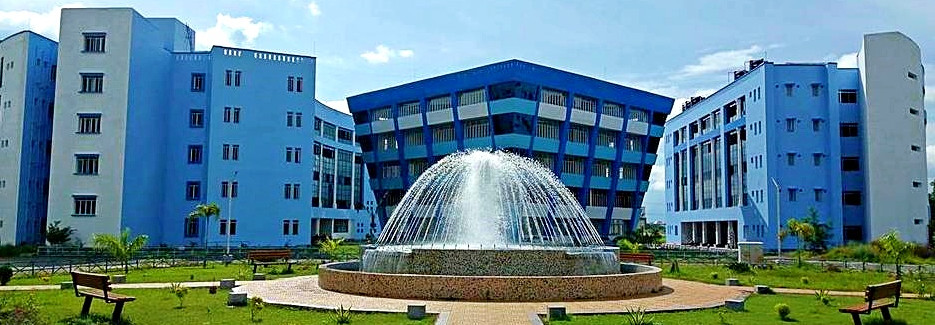
\includegraphics[width=0.5\textwidth]{makaut.jpg}
    \caption{An example figure.}
    \label{fig:fig_example}
\end{figure}

Tables are inserted similarly:
\begin{verbatim}
\begin{table}[h]
\centering
\begin{tabular}{|c|c|c|}
\hline
Column 1 & Column 2 & Column 3 \\
\hline
1 & 2 & 3 \\
4 & 5 & 6 \\
\hline
\end{tabular}
\caption{A simple table.}
\label{tab:example}
\end{table}
\end{verbatim}

% Class Notes for Day 4
\subsection{Class 4:}
\textbf{Topic: Cross-Referencing and Citations} \\

To cross-reference equations, figures, or sections in \LaTeX{}, you use the \verb|\label| and \verb|\ref| commands. For instance, Figure \ref{fig:fig_example} can be referenced like this.

You can automatically generate bibliographies using \texttt{BibTeX} or \texttt{BibLaTeX}, simplifying the citation process in academic documents.

\subsection{Compiling the Document}
To compile your \LaTeX{} document, you use a tool like \texttt{pdflatex}. Online editors like \textbf{Overleaf} make this process easier by providing an integrated environment for writing, compiling, and previewing your document.
